\documentclass{article}

\def\npart{III}
\def\nyear{2018}
\def\nterm{Michaelmas}
\def\nlecturer{Professor I.\ Smith}
\def\ncourse{Algebraic Topology}
\def\draft{Ongoing course, rough}
\ifx \nauthor\undefined
  \def\nauthor{Bhavik Mehta}
\else
\fi

\author{Based on lectures by \nlecturer \\\small Notes taken by \nauthor}
\date{\nterm\ \nyear}
\title{Part \npart\ -- \ncourse}

\usepackage[utf8]{inputenc}
\usepackage{amsmath}
\usepackage{amsthm}
\usepackage{amssymb}
\usepackage{enumerate}
\usepackage{mathtools}
\usepackage{graphicx}
\usepackage[dvipsnames]{xcolor}
\usepackage{tikz}
\usepackage{wrapfig}
\usepackage{centernot}
\usepackage{float}
\usepackage{braket}
\usepackage[hypcap=true]{caption}
\usepackage{enumitem}
\usepackage[colorlinks=true, linkcolor=mblue]{hyperref}
\usepackage[nameinlink,noabbrev]{cleveref}
\usepackage{nameref}
\usepackage[margin=1.5in]{geometry}

% Theorems
\theoremstyle{definition}
\newtheorem*{aim}{Aim}
\newtheorem*{axiom}{Axiom}
\newtheorem*{claim}{Claim}
\newtheorem*{cor}{Corollary}
\newtheorem*{conjecture}{Conjecture}
\newtheorem*{defi}{Definition}
\newtheorem*{eg}{Example}
\newtheorem*{ex}{Exercise}
\newtheorem*{fact}{Fact}
\newtheorem*{law}{Law}
\newtheorem*{lemma}{Lemma}
\newtheorem*{notation}{Notation}
\newtheorem*{prop}{Proposition}
\newtheorem*{question}{Question}
\newtheorem*{rrule}{Rule}
\newtheorem*{thm}{Theorem}
\newtheorem*{assumption}{Assumption}

\newtheorem*{remark}{Remark}
\newtheorem*{warning}{Warning}
\newtheorem*{exercise}{Exercise}

% \newcommand{\nthmautorefname}{Theorem}

\newtheorem{nthm}{Theorem}[section]
\newtheorem{nlemma}[nthm]{Lemma}
\newtheorem{nprop}[nthm]{Proposition}
\newtheorem{ncor}[nthm]{Corollary}
\newtheorem{ndef}[nthm]{Definition}

% Special sets
\newcommand{\C}{\mathbb{C}}
\newcommand{\N}{\mathbb{N}}
\newcommand{\Q}{\mathbb{Q}}
\newcommand{\R}{\mathbb{R}}
\newcommand{\Z}{\mathbb{Z}}

\newcommand{\abs}[1]{\left\lvert #1\right\rvert}
\newcommand{\norm}[1]{\left\lVert #1\right\rVert}
\renewcommand{\vec}[1]{\boldsymbol{\mathbf{#1}}}

\let\Im\relax
\let\Re\relax

\DeclareMathOperator{\Im}{Im}
\DeclareMathOperator{\Re}{Re}
\DeclareMathOperator{\id}{id}

\definecolor{mblue}{rgb}{0., 0.05, 0.6}


% preamble

\setcounter{section}{-1}

\usetikzlibrary{cd,decorations.pathmorphing,decorations.markings, fadings}
\tikzset{dot/.style = {circle,fill=black,inner sep=1pt}}

\DeclarePairedDelimiter\ceil{\lceil}{\rceil}
\DeclarePairedDelimiter\floor{\lfloor}{\rfloor}
\DeclareMathOperator{\image}{image}
\DeclareMathOperator{\im}{im}
\DeclareMathOperator{\Hom}{Hom}

%\newtheorem{manualtheoreminner}{Theorem}
%\newenvironment{manualtheorem}[1]{%
%    \renewcommand\themanualtheoreminner{#1}%
%    \manualtheoreminner
%}{\endmanualtheoreminner}

%\newcommand{\red}[1]{\textcolor{bred}{#1}}
%\newcommand{\green}[1]{\textcolor{bgreen}{#1}}
%\newcommand{\blue}[1]{\textcolor{bblue}{#1}}
%\newcommand{\yellow}[1]{\textcolor{byellow}{#1}}
%\newcommand{\orange}[1]{\textcolor{borange}{#1}}
%\newcommand{\purple}[1]{\textcolor{bpurple}{#1}}

% and here we go!

\begin{document}
\maketitle

\tableofcontents

\clearpage
\section{Introduction}
Algebraic topology concerns the connectivity properties of topological spaces.
Recall a space $X$ is \textbf{connected} if we cannot write $X = U \cup V$ where $U,V$ are non-empty, open and disjoint.
\begin{eg}
  $\mathbb{R}$ is connected (with its Euclidean topology), $\mathbb{R} \setminus \{0\}$ is not connected.
\end{eg}

\begin{cor}[Intermediate value theorem]
  If $f: \mathbb{R} \to \mathbb{R}$ is continuous and $f(x)>0, f(y) < 0$, then there is some $z$ lying between $x,y$ such that $f(z) = 0$.
\end{cor}
\begin{proof}
  If $f(z) \neq 0$ for all $z$, then $\mathbb{R} = f^{-1}(-\infty,0) \cup f^{-1}(0, \infty)$ is disconnected.
\end{proof}
For nice spaces, connected $\iff$ path-connected.
Recall: a space $X$ is path-connected if $\forall x,y \in X, \exists \gamma:[0,1] \to X$ continuous such that $\gamma(0) = x, \gamma(1) = y$.
Informally, any two maps of a point to $X$ can be continuously deformed into one another.
\begin{center}
  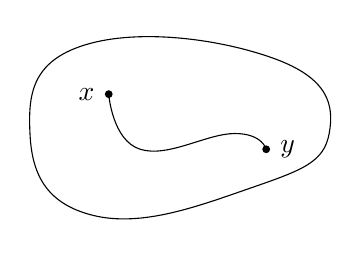
\begin{tikzpicture}[xscale=2]
    \draw plot [smooth cycle, tension=0.8] coordinates {(-180:1) (-120:1.2) (-60:0.8) (0:0.9) (60:1.1) (120:1.3)};
    \draw plot [smooth, tension=0.8] coordinates {(-0.5,0.5) (-0.3,-0.2) (0.3, 0) (0.5,-0.2)};
    \node [fill=black, circle, inner sep=1pt, label=left:$x$] at (-0.5,0.5) {};
    \node [fill=black, circle, inner sep=1pt, label=right:$y$] at (0.5,-0.2) {};
  \end{tikzpicture}
\end{center}
\begin{defi}[Homotopy]
  If $X,Y$ are topological spaces and $f,g : X \to Y$ are (continuous) maps, then $f$ is \textbf{homotopic} to $g$ if
  \begin{equation*}
    \exists F: X \times [0,1] \to Y
  \end{equation*}
  continuous such that
  \begin{equation*}
    F|_{X \times \{0\}} = f,
    F|_{X \times \{1\}} = g.
  \end{equation*}
  Write $f \simeq g$ or $f \simeq_F g$ and schematically
  \begin{center}
    \begin{tikzpicture}[scale=2]
      \draw (0,0) rectangle (1,1);
      \node at (0.5, 0.5) {$F$};
      \node at (0.5, -0.1) {$f$};
      \node at (0.5, 1.1) {$g$};
      \node (0) at (-0.2, 0) {$0$};
      \node (1) at (-0.2, 1) {$1$};
      \draw [->] (0) -- (1);
    \end{tikzpicture}
  \end{center}
\end{defi}

\begin{defi}[Simply connected]
  A path-connected space $X$ is \textbf{simply connected} if every two continuous maps $S^1 \to X$ are homotopic.
  Here $S^n = \set{x \in \mathbb{R}^{n+1} | \|x\| = 1}$ is the $n$ dimensional sphere, $S^1$ is the circle $\subseteq \mathbb{C}$.
\end{defi}
\begin{eg}
  $\mathbb{R}^2$ is simply connected but $\mathbb{R}^2 \setminus \{0\}$ is not. In fact, continuous maps $S^1 \xrightarrow{\gamma} \mathbb{R}^2 \setminus \{0\}$ have a degree $\deg(\gamma) \in \mathbb{Z}$, invariant under homotopy.
  (If $\gamma$ was differentiable, we could set $\deg(\gamma) = \frac{1}{2\pi i} \int_\gamma \frac{dz}{z} \in \mathbb{Z}$.)
  If $\gamma_n: S^1 \to \mathbb{R}^2 \setminus \{0\}$ has $t \mapsto e^{2\pi int}$ then $\deg(\gamma_n) = n$.
\end{eg}
\begin{cor}[Fundamental theorem of algebra]
  Every nonconstant complex polynomial has a root.
\end{cor}
\begin{proof}
  Let $f(z) = z^n + a_1 z^{n-1} + a_2 z^{n-2} + \dotsb + a_n$ be a complex polynomial and suppose $f(z) \neq 0 \ \forall z \in \mathbb{C}$. Let $\gamma_R(t) = f(R e^{2\pi it})$ so $\gamma_R : S^1 \to \mathbb{R}^2 \setminus \{0\}$.
  Now $\gamma_0$ is a constant map, so $\deg(\gamma_0) = 0$. By homotopy invariance of degree, $\deg(\gamma_R) = 0 \ \forall R$.

  If $R \gg \sum_i |a_i|$, we can consider $f_s(z) = z^n + s(a_1 z^{n-1} + \dotsb + a_n)$ for $0 \leq s \leq 1$, and on the circle $R e^{2\pi i t}$, $f_s$ also takes values in $\mathbb{R}^2 \setminus \{0\}$.
  If $\gamma_{R,s}(t) = f_s(R e^{2 \pi i t})$, then $\gamma_{R,1} = \gamma_R$ but $\gamma_{R,0} : z \mapsto z^n$, which has degree $n$.
  Now $\deg(\gamma_0) = \deg(\gamma_R) = \deg(\gamma_{R,1}) = \deg(\gamma_{R,0})$, so $n=0$ and $f$ is constant.
\end{proof}
\begin{fact}
  Any two maps $S^n \to \mathbb{R}^{n+1}$ are homotopic but maps $S^n \xrightarrow{f} \mathbb{R}^{n+1} \setminus \{0\}$ have a degree $\deg(f) \in \mathbb{Z}$, invariant up to homotopy.
  Moreover, the degree of the constant map is $0$ and the degree of inclusion is $1$.
\end{fact}
\begin{cor}[Brouwer's fixed point theorem]
  If $B^n = \set{x \in \mathbb{R}^n | \|x\| \leq 1}$, any continuous map $f: B^n \to B^n$ has a fixed point.
\end{cor}
\begin{proof}
  Suppose $f$ has no fixed point.
  Let $\gamma_R: S^{n-1} \to \mathbb{R}^n \setminus \{0\}$ be the map $v \mapsto R_v - f(R_v)$ for $0 \leq R \leq 1$. So $\gamma_0$ is a constant, so has degree 0.
  Hence $\deg(\gamma_1) = 0$.

  Let $\gamma_{1,s}(v) \coloneqq v - s f(v)$, for $0 \leq s \leq 1$ and $v \in S^{n-1}$.
  Note $\gamma_{1,s}$ has image in $\mathbb{R}^n \setminus \{0\}$: if $s=1$, this is because $v \neq f(v) \ \forall v$ and if $s < 1$ then $|v| > |s f(v)|$.
  Therefore $\gamma_1 = \gamma_{1,1}$ has the same degree as $\gamma_{1,0}$ which is the inclusion $S^{n-1} \hookrightarrow \mathbb{R}^n\setminus\{0\}$, a contradiction.
\end{proof}
\begin{defi}[Homotopy equivalence]
  We say spaces $X,Y$ are \textbf{homotopy equivalent} if $\exists$ maps $f : X \to Y$ and $g: Y \to X$ such that $g \circ f \simeq \id_X$ and $f \circ g \simeq \id_Y$. We write $X \simeq Y$.
\end{defi}
\begin{eg}\leavevmode
  \begin{itemize}
    \item Trivial case: if $X,Y$ are homeomorphic, i.e.\ $X \cong Y$, then clearly $X \simeq Y$.

    \item $\mathbb{R}^n \simeq \{0\}$, the single point. A space homotopy equivalent to a point is sometimes called contractible.
    \item $\mathbb{R}^n \setminus \{0\} \simeq S^{n-1}$.
      If $i: S^{n-1} \hookrightarrow \mathbb{R}^n \setminus \{0\}$ inclusion, and $p: \mathbb{R}^n \setminus \{0\} \to S^{n-1}$ is projection $v \mapsto \frac{v}{\|v\|}$, then $p \circ i = \id_{S^{n-1}}$ and $i \circ p \simeq \id_{\mathbb{R}^n \setminus \{0\}}$ via the homotopy
      \begin{align*}
        F: \mathbb{R}^n \setminus \{0\} \times [0,1] &\longrightarrow \mathbb{R}^n \setminus \{0\} \\
        (v,t) &\longmapsto t v + (1-t) \frac{v}{\|v\|}
      \end{align*}
  \end{itemize}
\end{eg}
Algebraic topology is the study of the set of spaces up to homotopy equivalence via the set of groups up to isomorphism.

The first naive attempt would be homotopy groups:
Loops (continuous maps $S^1 \to X$) with a common base-point can be concatenated and this induces a group structure on the set of homotopy classes of maps $(S^1, *) \to (X, x_0)$.
Recall this refers to continuous maps $S^1 \to X$ taking $* \mapsto x_0$ and a based homotopy $F : f \simeq g$ of two such is one such that $F |_{S \times \{t\}}$ sends $*$ to $x_0$ $\forall t$.

\begin{center}
  \begin{tikzpicture}[scale=0.9]
    \begin{scope}[decoration={markings,mark=at position 0.25 with {\arrow{>}}}]
      \draw [postaction={decorate}] (0,0) circle [radius=1cm];
      \draw [bred, postaction={decorate}] (4,1) circle [radius=1cm];
    \end{scope}
    \begin{scope}[decoration={markings,mark=at position 0.75 with {\arrow{<}}}]
      \draw [bblue, postaction={decorate}] (4,-1) circle [radius=1cm];
    \end{scope}
    \node [dot] at (0,-1) {};
    \node [dot] at (4,0) {};
    \draw [->, decorate, decoration={snake, post length=1pt}] (1.1, 0) -- (3.2, 0);
    \node at (2,-0.5) {concatenate};
    \draw [->] (4.8,0) to [bend right] (7,0);
    \node at (5.9, -0.6) {embed};

    \begin{scope}[xshift=8.8cm, scale=0.7]
      \draw (-1,0) to[bend left=40] (1,0);
      \draw (-1.2,0.15) to[bend right=40] (1.2,0.15);
      \draw ( 3,0) to[bend left=40] (5,0);
      \draw ( 2.8,0.15) to[bend right=40] (5.2,0.15);
      \draw [clip] plot [smooth cycle, tension=0.7] coordinates {
          (- 2.2, 0  )
          (- 1.5, 1  )
          (  0  , 1.4)
          (  2  , 1.1)
          (  4  , 1.4)
          (  5.5, 1  )
          (  6.2, 0  )
          (  5.5,-1  )
          (  4  ,-1.4)
          (  2  ,-1.1)
          (  0  ,-1.4)
          (- 1.5,-1  )
        };
      \node [dot] at (2,0) {};
      \begin{scope}[decoration={markings,mark=at position 0.5 with {\arrow{<}}}]
        \draw[bblue, postaction={decorate}] (2,0) to [out=180, in=22] (0.6,-0.2);
        \draw[bblue, postaction={decorate},dashed, very thin] (0.6,-0.2) to [out=202, in=-160] (1.2,-1.2);
        \draw[bblue, postaction={decorate}] (1.2,-1.2) to [out=20, in=-110] (2,0);
      \end{scope}
      \begin{scope}[decoration={markings,mark=at position 0.5 with {\arrow{>}}}]
        \draw[bred, postaction={decorate}] (2,0) to[out=0, in=170] (4,-0.8);
        \draw[bred, postaction={decorate}] (4,-0.8) to[out=-10, in=270] (5.7,0);
        \draw[bred, postaction={decorate}] (5.7,0) to [out=90, in=0] (4,0.9);
        \draw[bred, postaction={decorate}] (4,0.9) to[out=180,in=70] (2,0);
      \end{scope}
    \end{scope}

  \end{tikzpicture}
\end{center}

Again, there is a group structure on the set of based homotopy classes of maps $(S^n, *) \to (X, x_0)$ calld $\pi_n(X, x_0)$, the $n$-th homotopy group of $X$.
\begin{fact}
  $\{\pi_n(S^2, x)\}_{n \geq 1}$ is not known. Indeed, there is no simply connected manifold of dimension $> 0$ for which all $\pi_n$ are known.
\end{fact}

Instead, we will focus on homology theory, more precisely singular (co)homology.
We will obtain invariants of spaces in a two-step process:
\begin{enumerate}[label=(\alph*)]
  \item Associate to $X$ a chain complex (or cochain complex).
  \item take (co)homology of that complex.
\end{enumerate}
This will be rather computable for simple spaces. In this course, we will mostly focus on studying manifolds.
\begin{defi}[Chain complex, cochain complex]
  A \textbf{chain complex} $(C_*, d)$ is a sequence of abelian groups and homomorphisms
  \begin{equation*}
    \dots \longrightarrow C_{n+1} \overset{d_{n+1}}{\longrightarrow} C_n \overset{d_n}{\longrightarrow} C_{n-1} \overset{d_{n-1}}{\longrightarrow} C_{n-2} \longrightarrow \dots
  \end{equation*}
  (indexed by $\mathbb{N}$ or $\mathbb{Z}$) with the key property that $\forall n \ d_{n-1} \circ d_n = 0$
  Then $\image(d_{n+1}) \subseteq \ker(d_n)$ and the $n$-th homology group $H_n(C_*, d)$ of the chain complex is the quotient
  \begin{equation*}
    H_n(C_*, d) \coloneqq \frac{\ker(d_n)}{\im(d_{n+1})}.
  \end{equation*}

  A \textbf{cochain complex} $(C^*, d)$ is a sequence of abelian groups and homomorphisms
  \begin{equation*}
    \dots \longrightarrow C_{n+1} \overset{d_{n-1}}{\longrightarrow} C_n \overset{d_n}{\longrightarrow} C_{n+1} \longrightarrow \dots
  \end{equation*}
  such that $d^n \circ d^{n-1} \equiv 0 \ \forall n$
  The $n$-th cohomology group $H^n(C^*, d)$ is the quotient
  \begin{equation*}
    H^n(C^*, d) \coloneqq \frac{\ker(d^n)}{\im(d^{n-1})}.
  \end{equation*}
\end{defi}
\subsection{Singular (co)chains}
\begin{defi}[Simplex]\hypertarget{def:simplex}
  A \textbf{simplex} in a topological space $X$ is defined as follows.
  \begin{itemize}
    \item An $n$-simplex is the convex hull of $(n+1)$ ordered points $v_0, \dotsc, v_n$ in $\mathbb{R}^m$ such that $\set{v_i - v_0 | 1 \leq i \leq n}$ are linearly independent. Write this as $[v_0, \dotsc, v_n] = \sigma$.
  \end{itemize}
  The \textbf{standard $n$-simplex} is $\Delta^n = \set{(t_0, \dotsc, t_n) \in \mathbb{R}^{n+1} | \sum_{i=0}^n t_i = 1, t_i \geq 0 \ \forall i}$, e.g.
  \begin{center}
    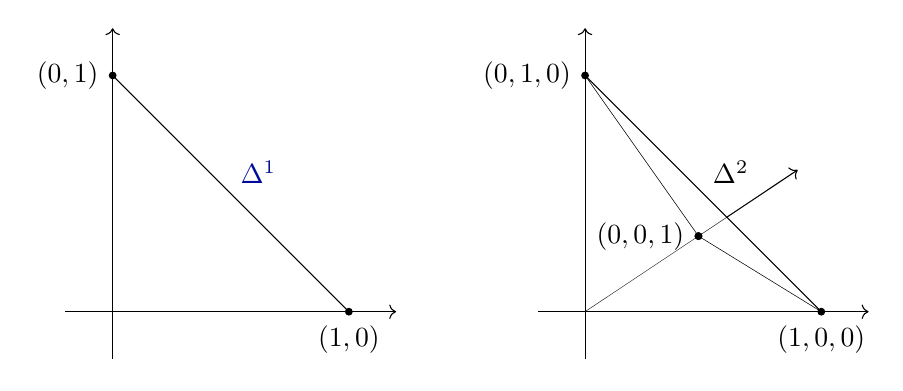
\begin{tikzpicture}[scale=3]
      \draw [->] (-0.2,0) -- (1.2,0);
      \draw [->] (0,-0.2) -- (0,1.2);
      \draw (1,0) -- (0,1);
      \node [dot, label={below:$(1,0)$}] at (1,0) {};
      \node [dot, label={left:$(0,1)$}] at (0,1) {};
      \node [mblue, above right] at (0.5,0.5) {$\Delta^1$};
      \begin{scope}[xshift=2cm]
        \draw [->] (-0.2,0) -- (1.2,0);
        \draw [->] (0,-0.2) -- (0,1.2);
        \draw (1,0) -- (0,1);
        \node [dot, label={below:$(1,0,0)$}] at (1,0) {};
        \node [dot, label={left:$(0,1,0)$}] at (0,1) {};
        \node [above right] at (0.5,0.5) {$\Delta^2$};
        \begin{scope}
          \draw [very thin, opacity=0.8] (0,0) -- (0.6,0.4);
          \draw [very thin] (1,0) -- (0.48,0.32);
          \draw [very thin] (0,1) -- (0.48,0.32);
          \node [dot, label={left:$(0,0,1)$}] at (0.48,0.32) {};
          \node [dot] at (0.48,0.32) {};
          \draw [->] (0.6,0.4) -- (0.9,0.6);
        \end{scope}
      \end{scope}
    \end{tikzpicture}

  \end{center}

\end{defi}

Note \emph{any} $n$-simplex is canonically the image of $\Delta^n$ under a linear homeomorphism $\Delta^n \to \sigma$ given by $(t_i) \mapsto \Sigma t_i v_i \in \sigma$.

An $n$ simplex in $X$ is a continuous map $\sigma: \Delta^n \to X$, or from any $n$-simplex to $X$.
Note any $n$-simplex has faces $\Delta_i^{n-1} \subseteq \Delta^n$ is defined by $\{t_i = 0\}$ and then this defines a corresponding face of any $\sigma$ via the map $\Delta^n \to \sigma$.
Write $i$th face of $\sigma$ as $[v_0, \dotsc, \hat{v_i}, \dotsc, v_n] \subseteq [v_0, \dotsc, v_n]$ (so a hat over a vertex means omit it).

Note the edges of any simplex are canonically oriented via `$v_i \to v_j$ if $i < j$'.

\begin{center}
  \begin{tikzpicture}
     %draw D1,D2,D3 (tetra) with arrows labelled

  \end{tikzpicture}
\end{center}
\begin{defi}[Singular chain complex]
  If $X$ is a space, the \textbf{singular chain complex} $C_*(X; \mathbb{Z})$ or just $C_*(X)$ is defined as follows:
  \begin{equation*}
    \Set{\sum_{i=1}^N h_i \sigma_i | N \in \mathbb{N}_{\geq 0}, h_i \in \mathbb{Z}, \sigma_i: \Delta^n \to X \text{ an $n$-simplex in $X$}}
  \end{equation*}
  the free abelian group on $n$-simplices in $X$.
\end{defi}
\begin{defi}[Boundary map]
  The boundary map $d: C_n(X) \to C_{n-1}(X)$ is defined by
  \begin{equation*}
    d \sigma = \sum_{i=0}^n (-1)^i \sigma|_{[v_0 \dotsm \hat{v_i} \dotsm v_n]}
  \end{equation*}
  on $\sigma=[v_0 \dotsm v_n]$ and extend to $C_n(X)$ by linearity.
\end{defi}
\begin{eg}
  For the simplex $\sigma = [v_0 v_1 v_2]$, $d(\sigma) = [v_0 v_1] - [v_0 v_2] + [v_1 v_2]$.
\end{eg}
\begin{lemma}
  $d^2 = 0$, i.e.\ $d_{n-1} \circ d_n= 0 \ \forall n$.
\end{lemma}
\begin{proof}
  \begin{align*}
    d \circ d(\sigma) &= d\left(\sum_{i=0}^n (-1)^i \sigma|_{[v_0 \dotsm \hat{v_i} \dotsm v_n]}\right)\\
                      &= \sum_{j < i} (-1)^i (-1)^j \sigma|_{[v_0 \dotsm \hat{v_j} \dotsm \hat{v_i} \dotsm v_n]}  \\
                      &+ \sum_{j > i} (-1)^i (-1)^{j+1} \sigma|_{[v_0 \dotsm \hat{v_i} \dotsm \hat{v_j} \dotsm v_n]}.
  \end{align*}
  Exchanging $i$ and $j$, these two terms exactly cancel.
\end{proof}
The resulting homology theory $H_*(X)$ or $H_*(X; \mathbb{Z})$ is called \textbf{singular homology}.

The $\mathbb{Z}$ keeps track of the fact that $h_i \in \mathbb{Z}$, we could similarly define $C_*(X, G)$ and $H_*(X,G)$ for any abelian group $G$.
Note $H_*(X,\mathbb{Z})$ is tautologically a homeomorphism invariant of $X$.

The idea is that $d$ takes the boundary of a region covered by simplices.

Elements of $\ker(d: C_i(X) \to C_{i-1}(X))$ are called cycles or $i$-cycles.
Elements in $\im(d)$ are called boundaries.

\begin{defi} [Cochain complex]
  The singular \textbf{cochain} complex of a space $X$, $C^*(X, \mathbb{Z})$ or $C^*(X)$, has cochain groups $C^n(X) \coloneqq \Hom(C_n(X), \mathbb{Z})$ and coboundary map $d^*: C^n(X) \to C^{n+1}(X)$ by $(d^* \psi)(\sigma) \coloneqq \psi(d \sigma)$. Here $\sigma \in C_{n+1}(X)$ and $d \sigma \in C_n(X)$, i.e.\ $d \sigma = d_{n+1} \sigma$.
\end{defi}
Observe $d^*(d^* \psi) (\sigma) = d^*(\psi|_{d \sigma}) = \psi|_{d \circ d(\sigma)}$ and $d \circ d(\sigma) = 0$, so $(d^*)^2 = 0$.
So indeed $(C^*(X), d^*)$ is a cochain complex and the cohomology $H^*(X,\mathbb{Z})$ or $H^*(X)$ is called \textbf{singular cohomology}.

Note $H^*(X,\mathbb{Z}) \neq \Hom_{\mathbb{Z}}(H_*(X,\mathbb{Z}),\mathbb{Z})$ in general.
Observe if $f: X \to Y$ is continuous and $\sigma: \Delta^n \to X$ is continuous, then I get $f \circ \sigma: \Delta^n \to Y$ is an $n$-simplex in $Y$, so I get
\begin{align*}
  f_*: C_*(X) &\to C_*(Y) \\
  f_*: C_n(X) &\to C_n(Y) \ \forall n
\end{align*}
are group homomorphisms.

Key observation: $df_* = f_*d$ since $f \circ (\sigma|_{[v_0 \dotsm \hat{v_i} \dotsm v_n]}) = (f \circ \sigma)|_{[v_0 \dotsm \hat{v_i} \dotsm v_n]}$
i.e.\ a continuous map $f: X \to Y$ induces a \textbf{chain map} of chain complexes
\begin{equation*}
  \begin{tikzcd}
    \dots \rar & C_{n+1}(X) \rar{d} \dar{f_*} & C_n(X) \rar{d} \dar{f_*} & C_{n-1}(X) \rar{d} \dar{f_*} & \dots \\
    \dots \rar & C_{n+1}(Y) \rar{d}  & C_n(Y) \rar{d}  & C_{n-1}(Y) \rar{d}  & \dots
  \end{tikzcd}
\end{equation*}
and each square commutes.
\begin{lemma}
  If $C_*$ and $D_*$ are chain complexes and $f_*:C_* \to D_*$ is a chain map, then $f_*$ indexes homomorphisms $f_*:H_i(C_*) \to H_i(D_*)$ for every $i$.
\end{lemma}
\begin{proof}
  Let $a \in H_i(C_*) = \frac{\ker(d_i:C_i \to C_{i-1})}{\im(d_{i+1}:C_{i+1} \to C_i)}$, so $a$ is represented by some $i$-cycle $\alpha \in C_i$, where $d \alpha = 0$.

  Then $f_*(d\alpha) = 0 = d(f_* \alpha) \implies f_*(\alpha) \in D_i$ is a cycle in the $D_*$-chain complex, and hence defines an element in $H_i(D_*) = \frac{\ker(d:D_i \to D_{i-1})}{\im(d:D_{i+1}\to D_i)}$. Call this element $b$ and set $f_*(a) = b$.
  This is well-defined.
  If $\alpha'$ also represents $a \in H_i(C_*)$, then $\alpha-\alpha'$ is a boundary, i.e.\ $\alpha-\alpha_i = d_{i+1}(\gamma)$ for some $\gamma \in C_{i+1}$.
  Then $f_*(\alpha) - f_*(\alpha') = f_*(d_{i+1}\gamma) = d_{i+1} f_*(\gamma)$ so $f_*(\alpha')$ and $f_*(\alpha)$ differ by a boundary, so define some element $b \in H_i(D_*)$.
  It is an easy exercise to check that this map $f_*:H_i(C_*) \to H_i(D_*)$ is indeed a homomorphism of groups.
\end{proof}
The upshot of this is that if $f:X\to Y$ is a continuous map of spaces, it induces maps $f_*:H_i(X) \to H_i(Y)$ for all $i$.
\begin{lemma}
  If $X \xrightarrow{f} Y \xrightarrow{g} Z$, then $(g \circ f)_* = g_* \circ f_*$, $id_* = id$.
\end{lemma}
\begin{proof}
  Exercise.
\end{proof}
In category-theoretic language, the association $X \mapsto H_*(X)$ is a functor from the category of topological spaces to the set of graded abelian groups.
Observe $f:X \to Y$ induces $f_*:C_*(X) \to C_*(Y)$ and this has an adjoint $f^*: C^*(Y) \to C^*(X)$.
Note this goes the other way. This again induces a map $H^*(Y) \to H^*(X)$.

\begin{lemma}
  \begin{equation*}
    H_*(\text{pt}) =
    \begin{cases*}
      \mathbb{Z} & * = 0\\
      0 & otherwise
    \end{cases*}
  \end{equation*}
\end{lemma}
\begin{proof}
  Note for each $n \geq0$, there is a \emph{unique} $n$-simplex in $X = $\{pt\}, namely the constant map $\sigma_n: \Delta^n \to $ \{pt\}.
  So the chain complex $(C_*(\text{pt}), d)$ is as follows.
  \begin{equation*}
    \begin{tikzcd}
      \dots \rar & C_n(X)
    \end{tikzcd}
  \end{equation*}
\end{proof}
\end{document}
